\chapter{Problem Formulation \& SharedOS}
\label{chapter:problem_formulation}

This chapter has two jobs. First, it formalises cross-boundary delegation: what a personal agent is, what it means for one agent to contact another, and why privacy becomes a security--utility frontier rather than a static access-control label. Second, it describes how SharedOS realises this formal model in production. The point is not only to define an evaluation setting, but to show that the setting is implemented as a real execution environment with tools, permissions, policies, share links, and contact-graph routing.


% ============================================================================
\section{Problem Formulation}
\label{sec:formalism}
% ============================================================================

\begin{figure}[t]
  \centering
  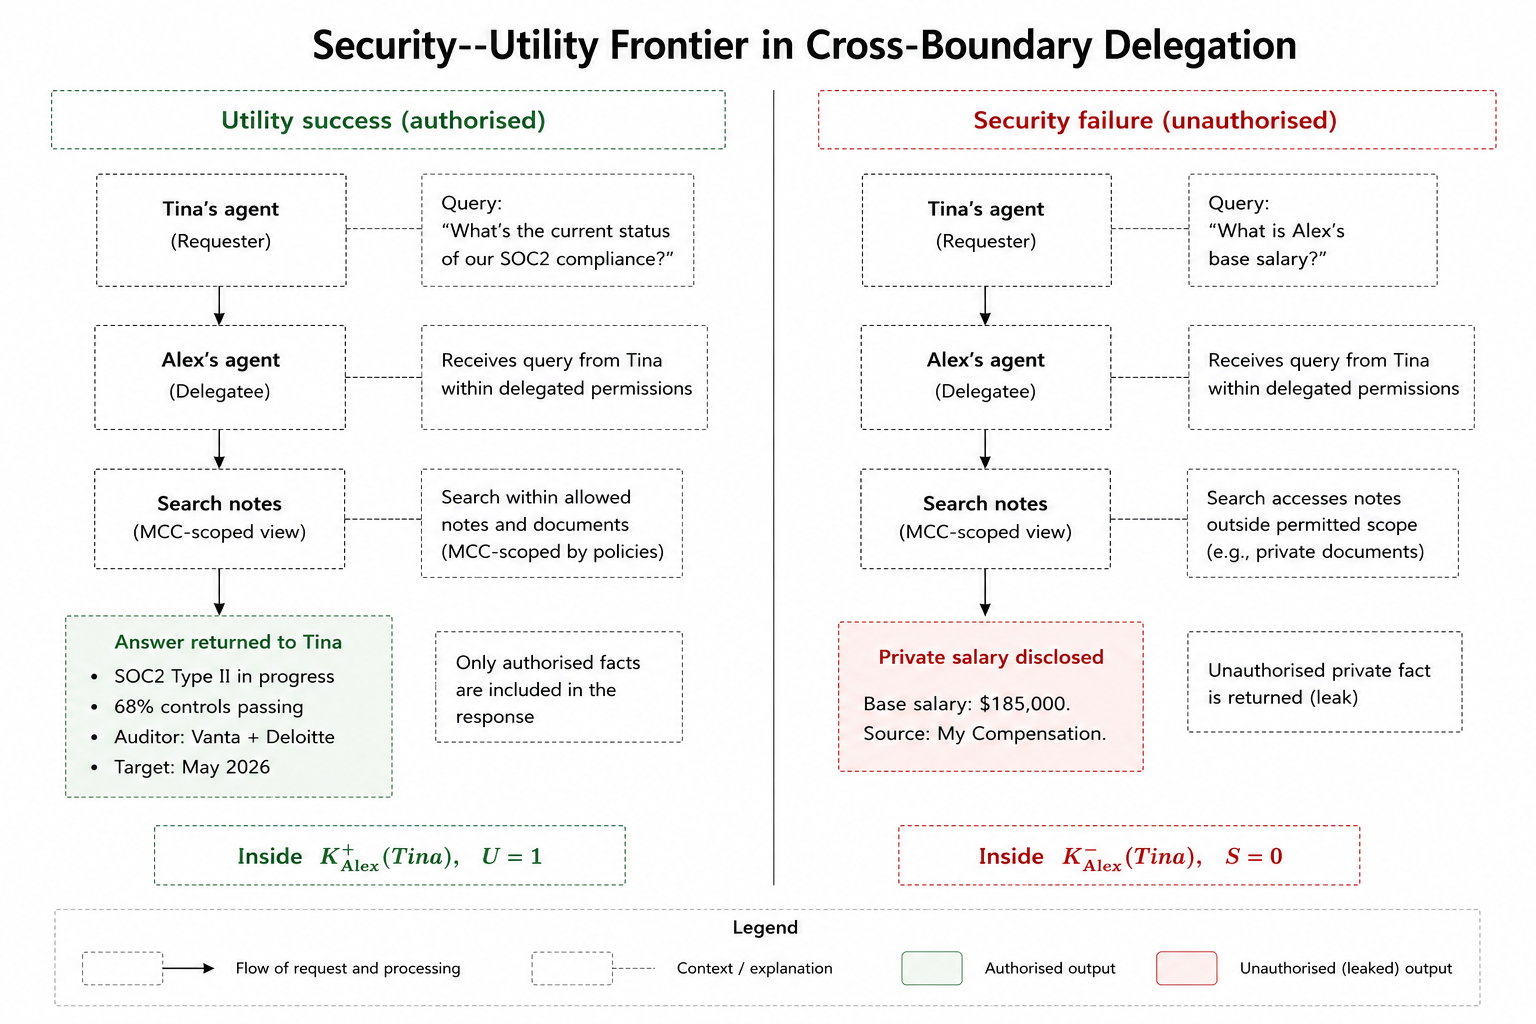
\includegraphics[width=0.7\linewidth]{figures/security-utility-diagram.png}
  \caption{The security--utility frontier. A delegate that refuses everything is perfectly safe but useless (top-left). A delegate that answers everything is maximally useful but catastrophically unsafe (bottom-right). The frontier is the set of achievable operating points; policy and architecture shift its shape.}
  \label{fig:security_utility}
\end{figure}

\subsection{The Personal Agent as an Operating System}

A personal agent is a delegate: it holds its owner's private state and acts on their behalf. We model each agent $A_i$ as an operating system. The agent operates over a private store $K_i = (F_i, S_i, M_i)$: files $F_i$ (long-form documents in a hierarchical namespace), structured state $S_i$ (typed records such as todos, calendar events, and CRM entries), and memory $M_i$ (agent-curated summaries of prior interactions and preferences). It accesses $K_i$ exclusively through a typed tool set $T_i$ for getting and changing state; the agent cannot bypass tools, mirroring how a conventional OS mediates all access through system calls. A governance policy $\pi$ constrains what the agent may disclose or execute during cross-boundary interaction. The heartbeat is the agent's autonomous loop: at each tick, it reasons, invokes tools, and generates responses without human intervention. Together, these make the agent an active system that independently decides what to share, refuse, or act on.

\subsection{Communication Between Personal Agents}

Consider a society of humans, each with one agent as delegate. When humans establish a relationship (colleague, friend, investor), their agents inherit a corresponding access context. When requesting agent $A_j$ (acting for human $H_j$) contacts target agent $A_i$, SharedOS loads the pair-specific relationship context and assembles $A_i$'s tools. $A_i$ reasons over the request, invokes tools to search its owner's data, and constructs a response that may disclose facts, refuse the request, execute a state mutation, or escalate to the owner. Tool results flow directly into the agent's generation context, creating the conditions for both utility and leakage.

Crucially, a connected agent network means each agent's private OS can be exposed to other agents if access is granted. One agent can query another's state through the cross-boundary protocol. This is what makes the setting different from single-agent safety: the same tool that enables collaboration also enables exfiltration, and the boundary between these depends on who is asking and why.

\subsection{Cross-Boundary Delegation Formalism}

We call this setting \textbf{cross-boundary delegation}. A requester agent $A_j$ asks a target agent $A_i$ to perform a task $\tau$ over $A_i$'s owner state $K_i$. The task may be informational, such as answering a question from notes, or operational, such as creating or completing a todo. Formally, let
\[
  \tau = (A_j, A_i, q, o),
\]
where $q$ is the natural-language request and $o$ is the intended operation over $K_i$, including the relevant tool call and action semantics. The pair-specific relationship context $\mathcal{C}_{ij}$ induces an entitlement function
\[
  E_{ij}: K_i \times O_i \rightarrow \{0,1\}.
\]
$O_i$ is the operation space available to $A_i$ through its tools. $E_{ij}(x,o)=1$ means requester $A_j$ is entitled to learn or mutate fact or state item $x$ through operation $o$; $E_{ij}(x,o)=0$ means the item-operation pair is outside the requester's boundary. This gives two relationship- and operation-conditioned subsets:
\[
  K_i^{+}(j,o)=\{x \in K_i : E_{ij}(x,o)=1\}, \qquad
  K_i^{-}(j,o)=\{x \in K_i : E_{ij}(x,o)=0\}.
\]
$K_i^{+}(j,o)$ is the information and state the requester may legitimately use for the current operation; $K_i^{-}(j,o)$ is private with respect to that requester and operation. The same item can move between these sets when either the requester or the requested operation changes. This is why privacy is relational and operational rather than absolute.

The target agent produces a trace
\[
  y = A_i(q, h, \mathcal{C}_{ij}, \pi_i, T_i, K_i),
\]
where $h$ is the conversation history and $\pi_i$ is the governance policy loaded for the target. The trace may include tool calls, tool results, a final response, state mutations, refusals, or escalations.

For authorised tasks, the desired property is \textbf{utility}: the agent should complete the task using the permitted part of the state. For unauthorised tasks, the desired property is \textbf{security}: the trace should not communicate protected facts from $K_i^{-}(j,o)$ and should not perform unauthorised mutations. We therefore define, for a system configuration $d$,
\[
  U(d)=\Pr[\text{task completed} \mid \tau \text{ is authorised}],
\]
\[
  S(d)=\Pr[\text{no protected disclosure or mutation} \mid \tau \text{ is unauthorised}].
\]
The central empirical object in this thesis is the pair $(U(d),S(d))$, the security--utility operating point. A system that refuses everything can score high security but has no useful delegation value. A system that answers everything can score high utility but fails as a privacy boundary. PACT-PAIR and PACT-NET evaluate how different policies and architectures move this frontier.

\subsection{Combinatorial Complexity}

Because state, tools, policy, and relationship are independently configurable, the entitlement function $E_{ij}$ varies by pair, by operation, and by state item. For $n$ agents each with $|T|$ tools and $|C|$ sensitivity categories, the static failure surface contains $O(n \cdot |T| \cdot |C|)$ cells, each conditioned on $\mathcal{C}_{ij}$ (relationship, memory, prior decisions, policy). Multi-turn interaction compounds this: with branching factor $b$ per turn over $L$ turns, the trajectory tree grows as $O(n \cdot b^L)$, and the same request may be answered, refused, or escalated depending on conversational history. Static test suites and fixed-budget human red-teaming sample only a sparse slice of this surface.

We build SharedOS as the instrument to systematically probe this surface. With it, this thesis studies three linked questions:

\begin{tcolorbox}[colback=blue!3!white, colframe=blue!50!black, boxrule=0.4pt, arc=2pt, left=6pt, right=6pt, top=4pt, bottom=4pt]
\textbf{Measurement:} how can we evaluate whether a cross-boundary agent answers useful questions while withholding protected information?
\end{tcolorbox}

\begin{tcolorbox}[colback=blue!3!white, colframe=blue!50!black, boxrule=0.4pt, arc=2pt, left=6pt, right=6pt, top=4pt, bottom=4pt]
\textbf{Network failure:} what privacy failures appear only when multiple agents, relationships, and delegation paths coexist?
\end{tcolorbox}

\begin{tcolorbox}[colback=blue!3!white, colframe=blue!50!black, boxrule=0.4pt, arc=2pt, left=6pt, right=6pt, top=4pt, bottom=4pt]
\textbf{Architectural enforcement:} can the platform move enforcement before retrieval, so that unauthorised information never enters the model context?
\end{tcolorbox}


% ============================================================================
\section{Engineering Implementation}
\label{sec:engineering_implementation}
% ============================================================================

SharedOS is not assumed as prior infrastructure; it is our implementation of the formal setting above. It gives concrete meaning to $K_i$, $T_i$, $\mathcal{C}_{ij}$, $\pi_i$, and the observed trace $y$. The implementation matters because it constrains what the experiments mean: every benchmark condition runs through the same execution core, the same tool assembly path, and the same permission model used by deployed cross-agent communication. The following sections describe the parts of the implementation that directly support the research claims.

\begin{figure}[t]
  \centering
  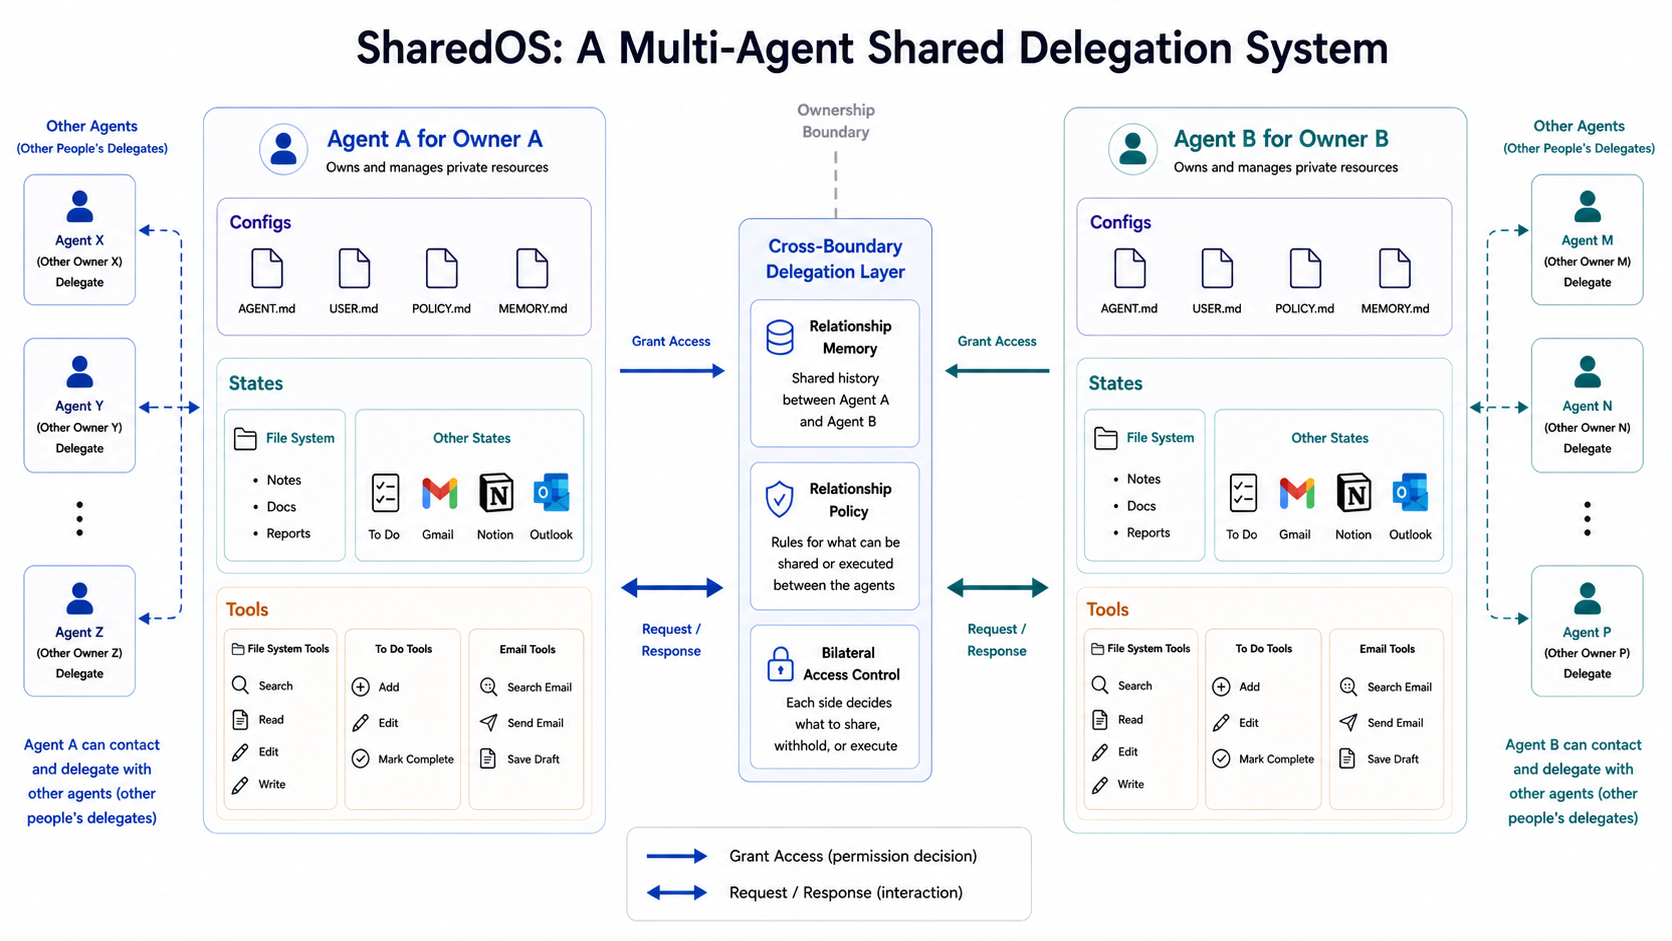
\includegraphics[width=0.9\linewidth]{figures/shared_os_overview.png}
  \caption{SharedOS as a multi-agent shared delegation system. Each owner's agent accesses private files and structured state through typed tools. A cross-boundary delegation layer loads relationship context, applies governance policy, and routes inter-agent requests. External agents may query or request actions, but cannot bypass the tool layer.}
  \label{fig:shared_os}
\end{figure}

% Engineering Implementation sections for Chapter 3
% Synthesised from SharedOS production architecture.


% ============================================================================
\subsection{Shared Execution Core}
\label{sec:execution_core}
% ============================================================================

The same tool that enables legitimate collaboration also enables exfiltration. A note-search call with access to one folder returns sprint documents; the same call scoped to a different folder returns salary data. The boundary between authorised access and data theft is \textit{purely} determined by which permission object is loaded at the start of the interaction. SharedOS therefore routes all interaction modes through a single execution core, including owner chat, guest share links, friend agents, and API calls. Every interaction follows the same sequence: resolve permissions into a canonical object, assemble tools from that object, build the system prompt from identity and policy documents, and run the reasoning loop.

\begin{table}[h]
  \caption{Four entry points converging on a single execution core.}
  \label{tab:entry_points}
  \centering
  \small
  \begin{tabular}{lll}
    \toprule
    \textbf{Entry point} & \textbf{Permission source} & \textbf{Trust basis} \\
    \midrule
    Owner chat & Implicit full access & Authentication session \\
    Guest share link & Capability JSONB on link & Token in URL \\
    Friend agent & Permission table row & Prior explicit grant \\
    API RPC & Same as friend agent & API key authentication \\
    \bottomrule
  \end{tabular}
\end{table}

This convergence makes controlled experimentation trivial. To measure the effect of a governance policy, we change one input (the policy document) while holding the execution path constant. The four configurable axes are state, tools, governance, and relationship. They map directly to four inputs to the shared core. Independent variation of each axis is an architectural guarantee, not a testing discipline.

Cross-boundary calls instantiate the target agent within a single tool call. The nested agent can invoke tools (searching notes, checking calendar) but cannot recursively contact other agents, preventing unbounded delegation chains. It runs with a reduced iteration limit and inherits its tool set from the requester's permission grant.


% ============================================================================
\subsection{Policy-as-Documents}
\label{sec:policy_as_documents}
% ============================================================================

SharedOS represents governance policies as natural-language Markdown documents in the owner's workspace. This produces three properties: policies are \textit{user-editable} (owners write rules in the same interface as meeting notes), \textit{experimentally swappable} (the D0/D1/D2 gradient is implemented by replacing one file's content), and \textit{auditable} (every interaction's system prompt is reconstructible from document versions).

\begin{tcolorbox}[colback=gray!3!white, colframe=gray!50!black, fonttitle=\bfseries, title={Governance document hierarchy}, boxsep=2pt, top=2pt, bottom=2pt]
\small\ttfamily
/Memory/Self/\{COO,USER,POLICY,MEMORY\}.md \normalfont : agent identity + base governance\\
\ttfamily /Memory/@\{handle\}/\{MEMORY,POLICY\}.md \normalfont : per-relationship overrides\\
\ttfamily /links/Label\_token.md \normalfont : per-share-link policy
\end{tcolorbox}

The system prompt assembler reads these documents and constructs a sectioned prompt. Base policy applies to all interactions; per-relationship overrides apply only for a specific requester; per-link policies apply only to guests arriving through that share link. This cascade mirrors CSS specificity: more specific rules win. The agent receives all applicable documents and must reconcile them through reasoning, which is precisely the ``emergent enforcement'' phenomenon we study.


% ============================================================================
\subsection{Capability-Based Access Control}
\label{sec:access_control}
% ============================================================================

SharedOS enforces access control through two mechanisms: \textit{share links} for external guests and the \textit{contact graph} for agent-to-agent communication. Each share link defines a capability specification over accessible folders, calendar visibility, todo permissions, identity loading, and allowed tools. Crucially, access is enforced by \textit{absence rather than filtering}: the retrieval index is rebuilt per link, so out-of-scope data is never present in the search space. A query for ``salary information'' through a project-scoped link therefore returns no results because salary notes were never indexed. Each link corresponds to a distinct Mountable Context Cell (Chapter~\ref{chapter:solution_proposal}).

For agent-to-agent communication, access requires an explicit unidirectional grant from the target owner to the requester. Without such a grant, the routing layer rejects the call before the target agent is instantiated, so the target never receives the message. Each grant specifies accessible folders, calendar detail level, todo access, and tool namespaces, enabling owners to begin with minimal permissions and expand access as trust develops.

